\thispagestyle{hoccungpinone}
\pagestyle{hoccungpi}
\everymath{\color{hoccungpi}}
\graphicspath{{../hoccungpi/pic/}}
\blfootnote{\color{hoccungpi}\color{hoccungpi}$^1$Giáo viên Toán trường THPT chuyên Lê Hồng Phong, Nam Định.}
\begingroup
\AddToShipoutPicture*{\put(0,616){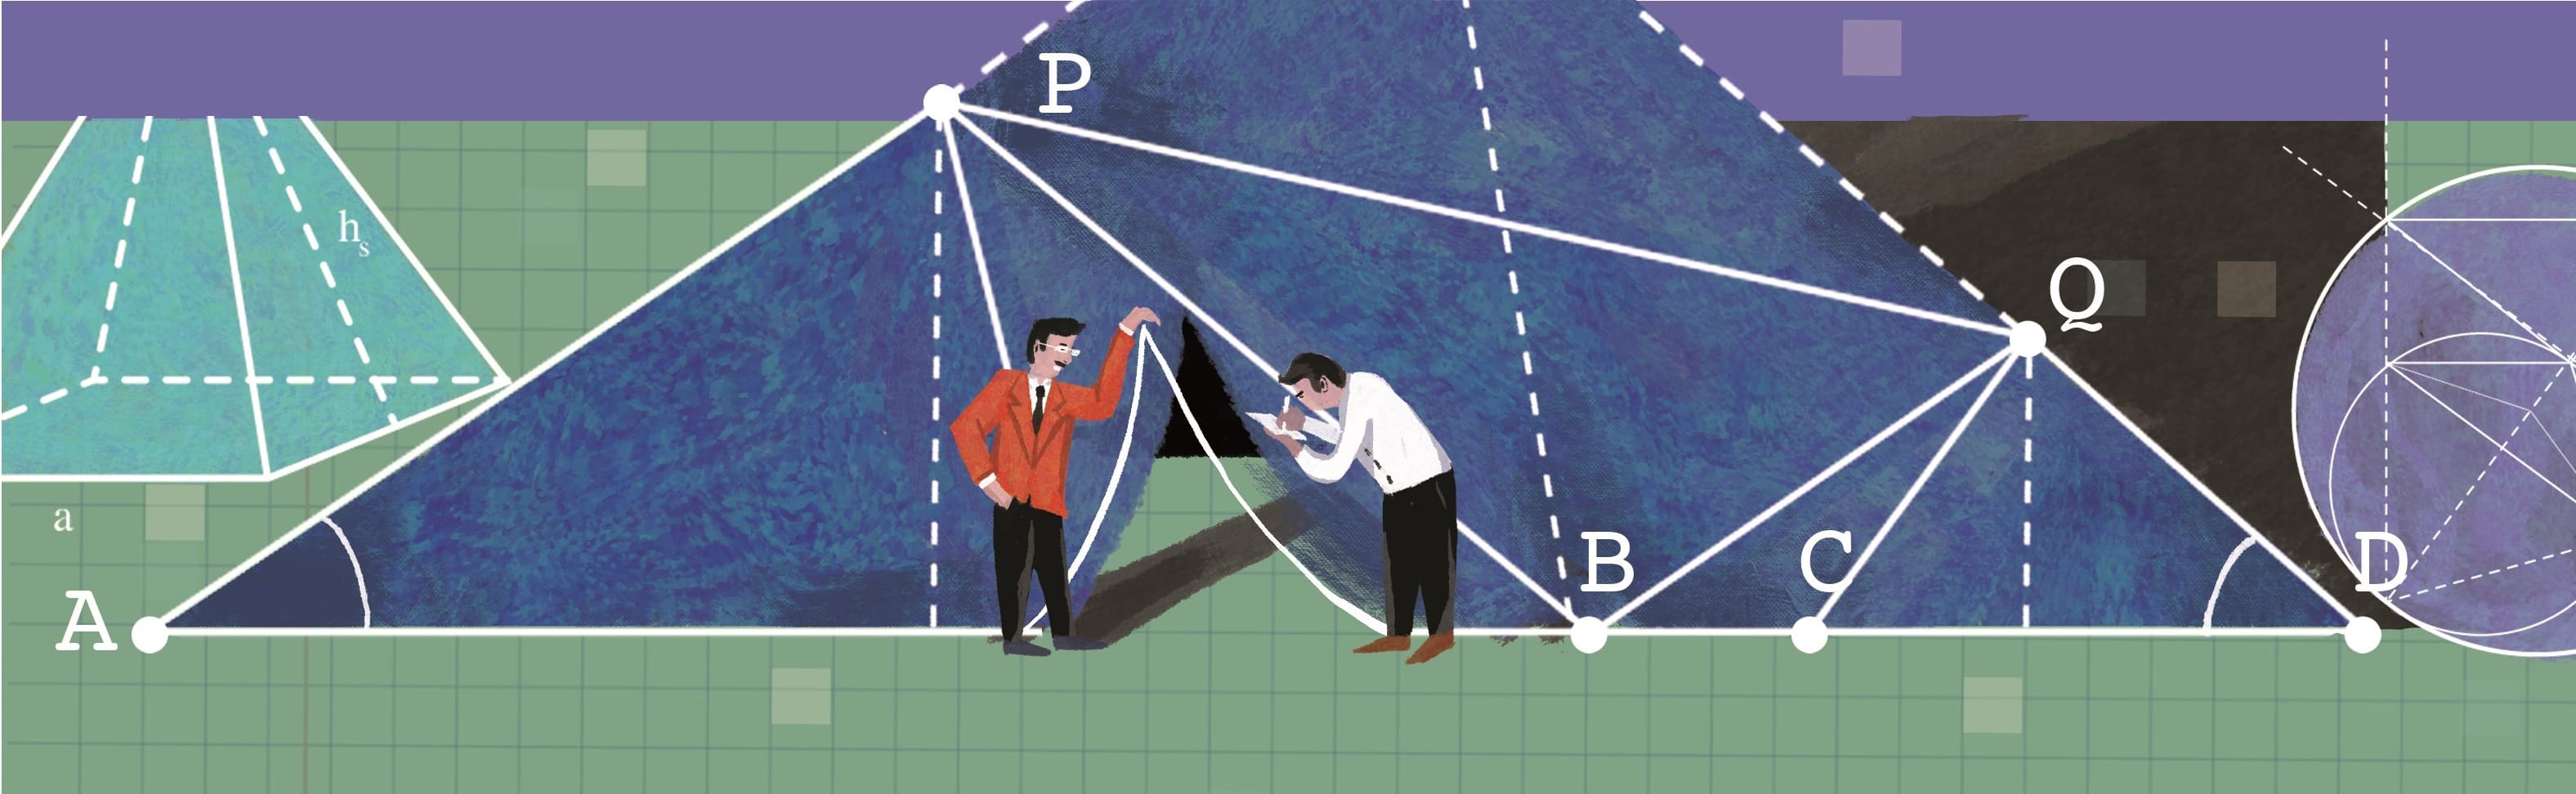
\includegraphics[width=19.3cm]{../bannerhoccungpi}}}
\AddToShipoutPicture*{\put(58,520){
\includegraphics[scale=1]{../tieude.pdf}}}
\centering
\endgroup
\vspace*{190pt}

\begin{multicols}{2}
	$\pmb{4.}$ \textbf{\color{hoccungpi}Đồ thị cây}
	\vskip 0.1cm
	Trong một số tình huống, ta có thể gặp những đồ thị mà số cạnh rất ít (còn gọi là đồ thị thưa). Khi đó, cấu trúc \textit{đồ thị cây} thường sẽ xuất hiện. Ta có định nghĩa về đồ thị cây như sau.
	\vskip 0.1cm
	\textbf{\color{hoccungpi}Định nghĩa} $\pmb{4.1}$ (Cây)\textbf{\color{hoccungpi}.}
	Một đồ thị được gọi là một \textit{cây} nếu nó liên thông và không chứa một chu trình nào. 
	\begin{figure}[H]
		\vspace*{-5pt}
		\centering
		\captionsetup{labelformat= empty, justification=centering}
		\definecolor{qqqqff}{rgb}{0.,0.,1.}
		\begin{tikzpicture}[scale=0.4, hoccungpi]
			\clip(3.52,0.5) rectangle (17.14,10.78);
			\draw [line width=1.2pt] (9.,1.)-- (9.,4.);
			\draw [line width=1.2pt] (9.,4.)-- (6.,7.);
			\draw [line width=1.2pt] (6.,7.)-- (4.,10.);
			\draw [line width=1.2pt] (6.,7.)-- (8.,10.);
			\draw [line width=1.2pt] (9.,4.)-- (12.,10.);
			\draw [line width=1.2pt] (9.,4.)-- (15.,7.);
			\draw [line width=1.2pt] (15.,7.)-- (13.,10.);
			\draw [line width=1.2pt] (15.,7.)-- (16.,10.);
			\begin{scriptsize}
				\draw [fill=qqqqff] (9.,1.) circle (5pt);
				\draw [fill=qqqqff] (9.,4.) circle (5pt);
				\draw [fill=qqqqff] (6.,7.) circle (5pt);
				\draw [fill=qqqqff] (4.,10.) circle (5pt);
				\draw [fill=qqqqff] (8.,10.) circle (5pt);
				\draw [fill=qqqqff] (12.,10.) circle (5pt);
				\draw [fill=qqqqff] (9.,4.) circle (5pt);
				\draw [fill=qqqqff] (15.,7.) circle (5pt);
				\draw [fill=qqqqff] (13.,10.) circle (5pt);
				\draw [fill=qqqqff] (16.,10.) circle (5pt);
			\end{scriptsize}
		\end{tikzpicture}
		\caption{\small\textit{\color{hoccungpi} Hình $5.$ Minh họa đồ thị cây.}}
		\vspace*{-10pt}
	\end{figure}
	Lưu ý rằng, một đồ thị cây không chứa chu trình, do đó nó không thể chứa một chu trình lẻ cạnh, hay một đồ thị cây cũng đồng thời là một đồ thị lưỡng phân. Nếu đồ thị $\pazocal{G}$ gồm một số thành phần liên thông, mà mỗi thành phần liên thông là một cây, thì $\pazocal{G}$ còn được gọi là một \textit{rừng}. Ta có định lý sau:
	\vskip 0.1cm 
	\textbf{\color{hoccungpi}Định lý} $\pmb{4.1}$ (Các đặc trưng tương đương của cây)\textbf{\color{hoccungpi}.}
	Cho  $\pazocal{G}$ là một đồ thị có $n$ đỉnh. Khi đó, các phát biểu sau là tương đương:
	\vskip 0.1cm
	$1.$ $\pazocal{G}$ là một cây;
	\vskip 0.1cm
	$2.$ $\pazocal{G}$ không có chu trình và có $n-1$ cạnh;
	\vskip 0.1cm
	$3.$ $\pazocal{G}$ liên thông và có $n-1$ cạnh;
	\vskip 0.1cm
	$4.$ $\pazocal{G}$ không có chu trình và nếu bổ sung vào một cạnh nối hai đỉnh không kề nhau thì xuất hiện một chu trình duy nhất;
	\vskip 0.1cm
	$5.$ $\pazocal{G}$ liên thông và nếu bỏ đi một cạnh bất kỳ thì $\pazocal{G}$ mất tính liên thông;
	\vskip 0.1cm
	$6.$ Mỗi cặp đỉnh trong $\pazocal{G}$ được nối với nhau bằng một đường đi duy nhất.
	\vskip 0.1cm
	Việc chứng minh định lý trên không khó. Bạn đọc quan tâm có thể tìm hiểu chi tiết chứng minh trong [$4$]. Để minh họa, chúng ta hãy cùng xét hai ví dụ sau.
	\vskip 0.1cm
	\textbf{\color{hoccungpi}Ví dụ} $\pmb{4.1}$ (Bài toán dự tuyển thi IMO  năm $2019$, Croatia đề xuất)\textbf{\color{hoccungpi}.}
	Trong một mạng xã hội, có $2019$ người dùng, một số họ là bạn của nhau (quan hệ bạn bè là quan hệ $2$ chiều). Ban đầu, có $1010$ người mà mỗi người có đúng $1009$ bạn và có $1009$ người mà mỗi người có đúng $1010$ bạn. Tuy nhiên, quan hệ bạn bè trong mạng này không bền vững, những sự kiện tương tự như sự kiện sau có thể lần lượt xảy ra (mỗi thời điểm chỉ có đúng một sự kiện xảy ra):
	\vskip 0.1cm
	Ký hiệu $A,B,C$ là ba người dùng sao cho $A$ là bạn của cả $B$ và $C$, nhưng $B$ và $C$ không phải là bạn của nhau. Khi đó $B$ và $C$ sẽ trở thành bạn, đồng thời $A$ không còn là bạn của cả $B$ và $C$.
	\vskip 0.1cm
	Chứng minh rằng, với mọi cấu hình ban đầu, tồn tại một dãy các sự kiện như sự kiện trên mà sau đó, mỗi người dùng chỉ còn tối đa một người bạn.  
	\vskip 0.1cm
	\textbf{\color{hoccungpi}Nhận xét. } Bài toán trên rõ ràng có thể phát biểu lại bằng ngôn ngữ của lý thuyết đồ thị như sau. Cho một đồ thị $\pazocal{G}$ có $2019$ đỉnh. Trong đó, $1010$ đỉnh có bậc $1009$ và $1009$ đỉnh có bậc $1010$. Ở mỗi bước, ta có thể: \textit{``Chọn ra ba đỉnh $A,B,C$ mà $A$ nối với cả $B$ và $C$; còn $B,C$ không nối với nhau. Sau đó, xóa hai cạnh $AB,AC$ và thêm cạnh $BC$ vào đồ thị $\pazocal{G}$.''}
	\vskip 0.1cm
	Gọi mỗi thao tác trên là một thao tác \textit{đảo cạnh}. Ta cần chứng minh rằng, thông qua một dãy các thao tác đảo cạnh, ta có thể tạo ra một đồ thị mà mỗi đỉnh của đồ thị có bậc không vượt quá $1$. Không khó để nhận ra, đây chính là một đồ thị rừng. 
	\vskip 0.1cm
	\textit{Lời giải.}
	Chú ý rằng một thao tác đảo cạnh bảo toàn tính chất: đồ thị $\pazocal{G}$ có ít nhất một đỉnh bậc lẻ và không phải là một đồ thị đầy đủ (tính chất này là hiển nhiên). Ta cũng chú ý rằng, đồ thị ban đầu là liên thông (chứng minh được dành cho bạn đọc như một bài tập). Bây giờ, ta mô tả một thuật toán gồm hai bước để chuyển đồ thị ban đầu về một đồ thị mà bậc của mỗi đỉnh không vượt quá $1$. 
	\vskip 0.1cm
	\textit{Bước $1$: Tồn tại một dãy các thao tác đảo cạnh để chuyển đồ thị ban đầu về một đồ thị dạng cây.}
	\vskip 0.1cm
	\textit{Chứng minh.} Vì số cạnh của đồ thị giảm đi $1$ sau mỗi thao tác đảo cạnh, ta chỉ cần chứng minh: chừng nào đồ thị $\pazocal{G}$ còn chứa một chu trình, thì tồn tại một thao tác đảo cạnh sao cho đồ thị mới được tạo ra vẫn liên thông. Ta đi chứng minh đồ thị chứa một chu trình $\pazocal{Z}$ và các đỉnh $A,B,C$ sao cho hai đỉnh $A$ và $B$ kề nhau trong chu trình $\pazocal{Z}$, đỉnh $C$ không nằm trong chu trình $\pazocal{Z}$ và kề với đỉnh $A$ nhưng không kề với đỉnh $B$. Bỏ hai cạnh $AB, AC$ và thêm cạnh $BC$ sẽ bảo toàn tính liên thông của đồ thị và khẳng định được chứng minh.  
	\begin{figure}[H]
		\vspace*{-5pt}
		\centering
		\captionsetup{labelformat= empty, justification=centering}
		\definecolor{qqqqff}{rgb}{0.,0.,1.}
		\begin{tikzpicture}[scale=0.25,hoccungpi]
			\draw (18.,30.)-- (12.,24.);
			\draw (12.,24.)-- (18.,18.);
			\draw (18.,18.)-- (26.,18.);
			\draw (26.,18.)-- (32.,24.);
			\draw (32.,24.)-- (26.,30.);
			\draw (26.,30.)-- (18.,30.);
			\draw (32.,24.)-- (38.,30.);
			\draw [dash pattern=on 2pt off 2pt] (26.,30.)-- (38.,30.);
			\draw (32.1,24.2) node[anchor=north west] {$A$};
			\draw (25.5,32) node[anchor=north west] {$B$};
			\draw (37.6,32) node[anchor=north west] {$C$};
			\begin{scriptsize}
				\draw [fill=qqqqff] (18.,30.) circle (5pt);
				\draw [fill=qqqqff] (12.,24.) circle (5pt);
				\draw [fill=qqqqff] (18.,18.) circle (5pt);
				\draw [fill=qqqqff] (26.,18.) circle (5pt);
				\draw [fill=qqqqff] (32.,24.) circle (5pt);
				\draw [fill=qqqqff] (26.,30.) circle (5pt);
				\draw [fill=qqqqff] (38.,30.) circle (5pt);
			\end{scriptsize}
		\end{tikzpicture}
		\caption{\small\textit{\color{hoccungpi}Hình $6.$ Nếu đồ thị $\pazocal{G}$ chứa chu trình $\pazocal{Z}$, thì ta vẫn có thể giảm số cạnh của nó.}}
		\vspace*{-10pt}
	\end{figure}
	Để tìm chu trình $\pazocal{Z}$ và các đỉnh $A,B,C$; ta sử dụng hai chiến lược sau. Nếu đồ thị $\pazocal{G}$ chứa một tam giác, ta xét một đồ thị con đầy đủ lớn nhất $K$. Rõ ràng $K$ chứa ít nhất ba đỉnh. Vì đồ thị $\pazocal{G}$ không là đồ thị đầy đủ, tồn tại một đỉnh $C$ không thuộc $K$ và kề với một đỉnh $A$ thuộc $K$. Do tính lớn nhất của $K$, có một đỉnh $B$ thuộc $K$ không kề với đỉnh $C$, và do đó ta có thể chọn chu trình $\pazocal{Z}$ trong $K$ và đi qua cạnh $AB$. 
	\vskip 0.1cm
	Nếu đồ thị $\pazocal{G}$ không chứa tam giác, ta xét một chu trình ngắn nhất $\pazocal{Z}$ trong đồ thị $\pazocal{G}$. Chu trình này không thể là một chu trình Hamilton (tức là chu trình đi qua tất cả các đỉnh của đồ thị, mỗi đỉnh đúng một lần). Thật vậy, nếu không, do tính nhỏ nhất của $\pazocal{Z}$, đồ thị $\pazocal{G}$ sẽ không chứa thêm một cạnh nào nữa, dẫn đến mỗi đỉnh của đồ thị $\pazocal{G}$ đều có bậc bằng $2$, mâu thuẫn với việc đồ thị luôn có đỉnh bậc lẻ. Như vậy, $\pazocal{Z}$ không là một chu trình Hamilton và vì thế có thể tìm được một đỉnh $C$ không thuộc $\pazocal{Z}$ và kề với một đỉnh $A$ thuộc $\pazocal{Z}$. Do đồ thị $\pazocal{G}$ không chứa tam giác, đỉnh $C$ sẽ không kề với bất kỳ đỉnh $B$ nào kề với $A$ trong $\pazocal{Z}$ và ta chọn được chu trình $\pazocal{Z}$ và ba đỉnh $A,B,C$.    
	\begin{figure}[H]
		\vspace*{-5pt}
		\centering
		\captionsetup{labelformat= empty, justification=centering}
		\definecolor{qqqqff}{rgb}{0.,0.,1.}
		\definecolor{cqcqcq}{rgb}{0.7529411764705882,0.7529411764705882,0.7529411764705882}
		\begin{tikzpicture}[scale=0.25, hoccungpi]
			\draw (18.,30.)-- (12.,24.);
			\draw (12.,24.)-- (18.,18.);
			\draw (18.,18.)-- (26.,18.);
			\draw (26.,18.)-- (32.,24.);
			\draw (32.,24.)-- (26.,30.);
			\draw (26.,30.)-- (18.,30.);
			\draw (32.,24.)-- (38.,30.);
			\draw [dash pattern=on 2pt off 2pt] (26.,30.)-- (38.,30.);
			\draw (32.1,24.2) node[anchor=north west] {$A$};
			\draw (25.5,32) node[anchor=north west] {$B$};
			\draw (37.6,32) node[anchor=north west] {$C$};
			\draw (18.,30.)-- (26.,18.);
			\draw (26.,30.)-- (18.,18.);
			\draw (12.,24.)-- (32.,24.);
			\draw (18.,30.)-- (18.,18.);
			\draw (26.,30.)-- (26.,18.);
			\draw (12.,24.)-- (26.,30.);
			\draw (26.,18.)-- (12.,24.);
			\draw (18.,30.)-- (32.,24.);
			\draw (32.,24.)-- (18.,18.);
			\begin{scriptsize}
				\draw [fill=qqqqff] (18.,30.) circle (5pt);
				\draw [fill=qqqqff] (12.,24.) circle (5pt);
				\draw [fill=qqqqff] (18.,18.) circle (5pt);
				\draw [fill=qqqqff] (26.,18.) circle (5pt);
				\draw [fill=qqqqff] (32.,24.) circle (5pt);
				\draw [fill=qqqqff] (26.,30.) circle (5pt);
				\draw [fill=qqqqff] (38.,30.) circle (5pt);
			\end{scriptsize}
		\end{tikzpicture}
		\caption{\small\textit{\color{hoccungpi} Hình $7.$ Minh họa cách tìm chu trình $\pazocal{Z}$ và ba điểm $A,B,C$.}}
		\vspace*{-10pt}
	\end{figure} 
	\textit{Bước $2$: Mọi đồ thị dạng cây đều có thể chuyển về một đồ thị có bậc mỗi đỉnh không vượt quá $1$ thông qua một dãy các thao tác đảo cạnh.}
	\vskip 0.1cm
	\textit{Chứng minh.} Để ý rằng thao tác đảo cạnh  bảo toàn tính chất không chứa chu trình. Do đó, kể từ một cây, sau các thao tác đảo cạnh, ta luôn có một đồ thị không chứa chu trình. Ngoài ra, mỗi thao tác đảo cạnh sẽ giảm số cạnh của đồ thị đi $1$ nên  đến một lúc nào đó ta không thể thực hiện thêm một thao tác đảo cạnh nào nữa. Khi này bậc của mỗi đỉnh của đồ thị này không vượt quá $1$. Thật vậy, nếu có một đỉnh $A$ với  kề với hai đỉnh $B,C$ nào đó (khi đó $B,C$ không kề nhau vì đồ thị đang xét không chứa chu trình) thì ta có thể thực hiện thêm một thao tác đảo cạnh.
	\vskip 0.1cm
	\textbf{\color{hoccungpi}Ví dụ} $\pmb{4.2}$ (Kỳ thi chọn đội tuyển Mỹ tham dự Egmo $2020$)\textbf{\color{hoccungpi}.} Cho $\pazocal{G}=(V,E)$ là một  đồ thị đơn có $n$ đỉnh. Một cạnh $e$ của của nó được gọi là một \textit{cạnh cổ chai} nếu có thể phân hoạch $V$ thành hai  tập $A,B$ thỏa mãn:
	\vskip 0.1cm
	$1.$ Có tối đa $100$ cạnh của $\pazocal{G}$ có một đầu mút thuộc $A$ và đầu mút còn lại thuộc $B$;
	\vskip 0.1cm
	$2.$ Cạnh $e$ là một trong số các cạnh như vậy.
	\vskip 0.1cm 
	Chứng minh rằng đồ thị $\pazocal{G}$ có tối đa $100(n-1)$ cạnh cổ chai.
	\vskip 0.1cm
	\textbf{\color{hoccungpi}Nhận xét. } Con số $100(n-1)$ ít nhiều gợi ý cho ta $100$ cấu trúc cây trong đồ thị $\pazocal{G}$. 
	\vskip 0.1cm
	\textit{Lời giải.} Gọi $F_1$ là một rừng lớn nhất trong $\pazocal{G}$ (nếu $\pazocal{G}$ liên thông thì $F_1$ chính là một cây). Xóa đi các cạnh của $F_1$ và gọi $F_2$ là rừng lớn nhất trong đồ thị mới nhận được (vẫn có $n$ đỉnh). Cứ tiếp tục như vậy, cho đến $F_{100}$ là rừng lớn nhất trong đồ thị nhận được khi xóa đi các cạnh của  $F_1\cup F_2\cup \cdots \cup F_{99}$. Giả sử ngược lại, $\pazocal{G}$ có nhiều hơn $100(n-1)$ cạnh cổ chai. Mỗi rừng $F_i$ (với $i=1,\dots,100$) (có $n$ đỉnh) có tối đa $n-1$ cạnh. Do vậy, tổng số các cạnh trong $F_1\cup F_2\cup \cdots \cup F_{100}$ không vượt quá $100(n-1)$. Vì vậy, vẫn tồn tại một cạnh cổ chai không nằm trong bất kỳ $F_{i}, i=1, 2, \ldots, 100$ nào.
	Gọi $x-y$ là một cạnh như vậy ($x,y$ là hai đỉnh của đồ thị). Rõ ràng, trong mỗi $F_i$, có một đường đi từ $x$ đến $y$ vì nếu không, thêm cạnh $x-y$ vào $F_i$ ta vẫn có một rừng (mâu thuẫn với cách chọn $F_i$ lớn nhất). Vì vậy, trong $\pazocal{G}$ có ít nhất $101$ đường đi từ $x$ đến $y$, hơn nữa hai đường đi bất kỳ đều không có cạnh chung. Tuy nhiên, khi đó cạnh $x-y$ không thể là cạnh cổ chai. Thật vậy, gọi $A,B$ là phân hoạch của $V$ tương ứng với cạnh cổ chai $x-y$. Với mỗi $i$, đường đi  trong $F_i$ từ $x$ đến $y$ phải chứa một cạnh nối một đỉnh thuộc $A$ và một đỉnh thuộc $B$. Tóm tại, ta tìm được $101$ cạnh của $G$ mà một đầu mút thuộc $A$ và  đầu mút còn lại thuộc $B$ (mâu thuẫn với điều kiện $(1)$). 
	\vskip 0.1cm
	Hy vọng rằng qua một số lý thuyết và bài tập minh họa, bạn đọc đã ít nhiều thấy được tiềm năng, sự phong phú và mối liên hệ của lý thuyết đồ thị với nhiều mảng kiến thức khác. Rõ ràng, khi mô hình hóa được một bài toán dưới dạng ngôn ngữ đồ thị, ta có thể tìm ra định hướng tốt trong việc tìm kiếm lời giải. Cụ thể hơn, khi gặp một mô hình đồ thị có nhiều cạnh, ta có thể liên tưởng đến cấu trúc đồ thị lưỡng phân; ngược lại, một mô hình đồ thị ít cạnh làm chúng ta liên tưởng đến đồ thị dạng cây, rừng.  
	Phần cuối của bài viết này là một số bài tập giúp rèn luyện thêm kỹ năng phát hiện và sử dụng các cấu trúc đồ thị lưỡng phân và cây.   
	\vskip 0.1cm
	$\pmb{5.}$ \textbf{\color{hoccungpi}Một số bài toán tự rèn luyện}
	\vskip 0.1cm
	\textbf{\color{hoccungpi}Bài $\pmb{1.}$} \textit{(Olympic Canada năm $2020$)} Cho đồ thị $\pazocal{G}$ có $19998$ đỉnh. Mỗi đồ thị con gồm $9999$ đỉnh của $\pazocal{G}$ đều chứa ít nhất $9999$ cạnh. Hỏi $\pazocal{G}$ có ít nhất bao nhiêu cạnh?
	\vskip 0.1cm
	\textbf{\color{hoccungpi}Bài $\pmb{2.}$}\textit{(Mở rộng Bài $2$)}  Cho đồ thị $\pazocal{G}$ có $2n$ đỉnh. Mỗi đồ thị con $n$ đỉnh của  $\pazocal{G}$ đều có ít nhất $n$ cạnh. Chứng minh rằng $\pazocal{G}$ có ít nhất $5n$ cạnh.
	\vskip 0.1cm
	\textbf{\color{hoccungpi}Bài $\pmb{3.}$} \textit{(Olympic Liên bang Nga năm $2004$)} Một quốc gia có $1001$ thành phố.  Hai thành phố bất kỳ được nối với nhau bằng một con đường một chiều. Mỗi thành phố có $500$ con đường đi ra và $500$ con đường đi vào. Có một tổ chức ly khai xuất hiện và chiếm đóng $668$ thành phố. Chứng minh rằng, trong khu vực ly khai này, từ mỗi thành phố đều có có thể đi đến một thành phố khác.
	\vskip 0.1cm
	\textbf{\color{hoccungpi}Bài $\pmb{4.}$}  Cho đồ thị $\pazocal{G} = (V,E)$ thỏa mãn $|E| = |V| +4$. Chứng minh rằng, trong $\pazocal{G}$ có
	hai chu trình không có cạnh chung. 
	\vskip 0.1cm
	\textbf{\color{hoccungpi}Tài liệu}
	\vskip 0.1cm
	[$1$] Đỗ Đức Thái, \textit{Chuyên đề học tập toán $11$}. NXB Đại học Sư phạm Hà Nội. 
	\vskip 0.1cm
	[$2$] Hà Huy Khoái, \textit{Chuyên đề học tập toán $11$}. NXB Giáo dục Việt Nam. 
	\vskip 0.1cm
	[$3$] Asratian, Armen S.; Denley, Tristan M. J.; Häggkvist, Roland, \textit{Bipartite Graphs and their Applications}. Cambridge University Press, $1998$.
	\vskip 0.1cm
	[$4$] Bender, Edward A.; Williamson, S. Gill , \textit{Lists, Decisions and Graphs  With an Introduction to Probability}, $2010$.
	\vskip 0.1cm
	[$5$] Titu Andreescu, Bogdan Enescu, \textit{Mathematical Olympiad Treasures}. Springer, $2011$.
	\vskip 0.1cm                 
	[$6$] Website \url{https://artofproblemsolving.com}. 
\end{multicols}